\documentclass[colorlinks]{docs}

% 1. PDF verzió kezelése (a figyelmeztetés megszüntetéséhez)
\pdfminorversion=7

% 2. Magyar nyelv specifikus beállítások (a babel ELŐTT)
\PassOptionsToPackage{defaults=hu-min}{magyar.ldf}

% 3. Alapvető kódolás és nyelvi csomag
\usepackage[T1]{fontenc}
\usepackage[utf8]{inputenc}
\usepackage[magyar]{babel}

% 4. Minden egyéb csomag duplikáció nélkül
\usepackage{graphicx,amsmath,amssymb,amsthm,hulipsum,bussproofs}
\usepackage{listings,xcolor,rotating,booktabs,fancyvrb}
\usepackage[normalem]{ulem}
\usepackage{pdfpages}
\usepackage[linguistics]{forest}
\usepackage{stackengine,scalerel}
\usepackage{url}
\def\UrlBreaks{\do\/\do-\do\.\do\a\do\b\do\c\do\d\do\e\do\f\do\g\do\h\do\i\do\j\do\k\do\l\do\m\do\n\do\o\do\p\do\q\do\r\do\s\do\t\do\u\do\v\do\w\do\x\do\y\do\z\do\0\do\1\do\2\do\3\do\4\do\5\do\6\do\7\do\8\do\9}
% Formázási és matematikai beállítások
\footnotestyle{rule=fourth}
\DeclareMathOperator{\tg}{tg}
\newtheorem{tetel}{Tétel}[chapter]
\newtheorem{lemma}[tetel]{Lemma}
\theoremstyle{definition}
\newtheorem{definicio}[tetel]{Definíció}
\newtheorem{feladat}[tetel]{Feladat}
\theoremstyle{remark}
\newtheorem{megjegyzes}[tetel]{Megjegyzés}
\newtheorem*{megoldas}{Megoldás}

% Listings beállítása a magyar karakterekhez
\lstset{
	inputencoding=utf8,
	extendedchars=true,
    literate={á}{{\'a}}1 {é}{{\'e}}1 {í}{{\'i}}1 {ó}{{\'o}}1 {ö}{{\"o}}1 {ő}{{\H{o}}}1
    {ú}{{\'u}}1 {ü}{{\"u}}1 {ű}{{\H{u}}}1
    {Á}{{\'A}}1 {É}{{\'E}}1 {Í}{{\'I}}1 {Ó}{{\'O}}1 {Ö}{{\"O}}1 {Ő}{{\H{O}}}1
    {Ú}{{\'U}}1 {Ü}{{\"U}}1 {Ű}{{\H{U}}}1,
    breaklines=true,
    basicstyle=\ttfamily\small,
    keywordstyle=\color{blue},
    commentstyle=\color{gray},
    stringstyle=\color{teal}
}


% Define JavaScript language for listings
\lstdefinelanguage{JavaScript}{
    keywords={break, case, catch, continue, debugger, default, delete, do, else, finally, for, function, if, in, instanceof, new, return, switch, this, throw, try, typeof, var, void, while, with, let, const, export, import, await, async},
    ndkeywords={class, export, boolean, throw, implements, import, this, new},
    sensitive=true,
    comment=[l]{//},
    morecomment=[s]{/*}{*/},
    morestring=[b]',
    morestring=[b]",
    alsoletter={-},
    alsodigit={:},
    morekeywords=[2]{=>, yield, async, await, constructor},
    keywordstyle=\color{blue}\bfseries,
    ndkeywordstyle=\color{green}\bfseries,
    identifierstyle=\color{black},
    commentstyle=\color{gray}\ttfamily,
    stringstyle=\color{red}\ttfamily,
}

% Customize listings appearance
\lstset{
    language=JavaScript,
    extendedchars=true,
    inputencoding=utf8,
    basicstyle=\ttfamily\small,
    numbers=left,
    numberstyle=\tiny\color{gray},
    stepnumber=1,
    numbersep=10pt,
    showstringspaces=false,
    breaklines=true,
    frame=single,
    captionpos=b,
    escapeinside={\%*}{*)},
}

% Fordított 'T' szimbólum definiálása
\def\tang{\ThisStyle{\abovebaseline[0pt]{\scalebox{-1}{$\SavedStyle\perp$}}}}

\begin{document}

\title{Synk}

\author{Erdős Martin\\Makkai Krisztián\\Szedlák Krisztián\\Szoftverfejlesztő és -tesztelő szak}
\institute{Informatika és távközlés ágazat}
\supervisor{Kerényi Róbert Nándor\\oktató}
\city{Miskolc}
\date{2026}
\maketitle

\tableofcontents
\newpage

% --- 1. fejezet ---
\chapter{Bevezetés}

\section{A projekt bemutatása és célja}
A \textbf{Synk} egy innovatív, többplatformos koncertjegy-értékesítési ökoszisztéma. A projekt célja egy olyan integrált környezet létrehozása, amely a modern webes technológiák, az asztali alkalmazások ereje és a mobilis megoldások rugalmassága révén szolgálja ki a rendezvényszervezői piacot. A rendszer alapvető küldetése a jegyvásárlási folyamat transzparenssé tétele, a valós idejű készletkezelés és a biztonságos, digitális jegyfelhasználás biztosítása.

A Synk architektúrája négy fő pillérre épül: egy villámgyors vásárlói webfelületre, egy robusztus adminisztrációs asztali alkalmazásra, egy hordozható mobilalkalmazásra és az ezeket kiszolgáló központi API-ra.



\begin{figure}[ht!]
	\centering
	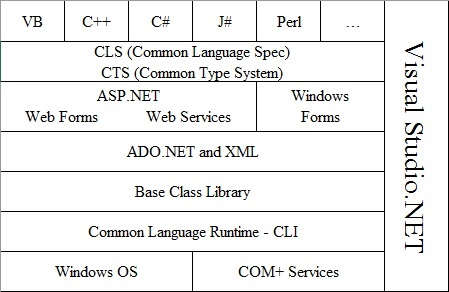
\includegraphics[width=9cm]{figures/dotNET.jpg}
	\caption[dotNET]{A Synk szoftverarchitektúrája}
	\label{fig-dotNET}
\end{figure}

\section{Célközönség meghatározása}
A szoftver célközönsége rétegzett, minden felhasználói típushoz dedikált felület tartozik:
\begin{itemize}
    \item \textbf{Végfelhasználók (Vásárlók):} A Next.js felületen böngésznek, a React Native mobilalkalmazásban pedig tárolják és kezelik digitális jegyeiket.
    \item \textbf{Rendezvényszervezők:} A webfelületen / WPF kliensen keresztül végzik a komplex eseménymenedzsmentet és felhasználókezelést.
    \item \textbf{Helyszíni személyzet:} A mobilalkalmazás speciális funkcióival végzik a gyors, QR-kód alapú jegyérvényesítést.
\end{itemize}

Az automatikus tételbizonyítás egyik fontos megközelítése Herbrand nevéhez fűződik (1930). Herbrand algoritmust dolgozott ki olyan interpretáció előállítására, amely hamissá tehet egy formulát. Ugyanakkor, ha az illető formula logikailag igaz, tehát nincs olyan interpretáció, amelyben hamissá válna, ez az algoritmus véges sok lépés után megáll. {\cite{Varteresz}} Ez a logikai szigor alapvető a Synk jegyfoglalási algoritmusánál is, ahol el kell kerülni az olyan állapotokat, amelyek ellentmondáshoz (pl. túlfoglaláshoz) vezetnének.

\section{Alkalmazott technológiák és eszközök}
Lásd: \ref{fig-melleklet1} melléklet ábrát.

\begin{itemize}
	\item \textbf{Adatbázis:} PostgreSQL \cite{postgresql} – A komplex relációs adatok és tranzakciók biztonságos kezeléséhez.
	\item \textbf{Backend:} RESTful API (ASP.NET Core) \cite{dotnet10} – A központi üzleti logika kiszolgálója.
	\item \textbf{Webes kliens:} Next.js \cite{nextjs} – Szerveroldali rendereléssel támogatott React keretrendszer az optimális SEO és sebesség érdekében.
	\item \textbf{Mobil alkalmazás:} React Native (Expo) \cite{reactnative} – Cross-platform megoldás, amely lehetővé teszi a natív élményt iOS és Android eszközökön a digitális jegyek kezeléséhez.
	\item \textbf{Asztali kliens:} WPF (C\#) \cite{gossman2005} – Nagy teljesítményű adminisztrációs felület Windows környezetbe.
	\item \textbf{Gyorsítótár:} Redis \cite{redis} – Nagy teljesítményű in-memory kulcs-érték tároló a munkamenetek és adatok gyors eléréséhez.
	\item \textbf{Objektumtároló:} MinIO \cite{minio} – S3-kompatibilis nyílt forráskódú objektumtároló a médiafájlok és jegy PDF-ek kezeléséhez.
\end{itemize}

% --- 2. fejezet ---
\chapter{Követelményanalízis}

\section{Funkcionális követelmények}
A Synk rendszer funkcionális követelményei a tier-alapú jegyértékesítési modellre és a többrétegű kliensarchitektúrára fókuszálnak.

\subsection{Webes felület (Next.js)}
\begin{itemize}
    \item \textbf{Események listázása:} A koncertek adatlapjának megjelenítése (leírás, dátum, fellépők).
    \item \textbf{Tier-alapú jegyválasztás:} A felhasználó választhat a különböző árkategóriájú és szolgáltatástartalmú jegytípusok (pl. Early Bird, Standard, VIP) közül a szabad készlet erejéig.
    \item \textbf{Jegylistázás:} Biztonságos jegykezelés, PDF formátumú jegyletöltés.
\end{itemize}

\subsection{Mobil alkalmazás (React Native + Expo)}
\begin{itemize}
    \item \textbf{Jegyek kezelése:} A megvásárolt, különböző kategóriájú jegyek tárolása és vizuális megjelenítése.
    \item \textbf{QR-kódos validáció:} Egyedi, dinamikusan generált azonosítók megjelenítése a belépéshez.
    \item \textbf{Beléptető modul:} A személyzet számára elkülönített felület a jegyek szkennelésére és valós idejű érvénytelenítésére az API-n keresztül.
\end{itemize}

\subsection{Adminisztrációs kliens (WPF)}
A WPF alkalmazás kizárólag belső, adminisztratív célokat szolgál, közvetlen elérést biztosítva az üzleti adatokhoz:
\begin{itemize}
    \item \textbf{Rendszerfelügyelet:} Felhasználó, és felhasználói jogosultságok kezelése és az adatbázis integritásának ellenőrzése.
\end{itemize}

\section{Nem funkcionális követelmények}
\begin{itemize}
    \item \textbf{Tranzakcionális biztonság:} A PostgreSQL ACID tulajdonságait kihasználva garantálni kell, hogy a jegy-tierek darabszáma (stock) ne csökkenhessen negatív tartományba párhuzamos vásárlások esetén sem.
    \item \textbf{Keresőoptimalizálás (SEO):} A Next.js használatával biztosítani kell az eseményoldalak gyors indexelhetőségét.
    \item \textbf{Hordozhatóság:} A React Native kódalapnak minimális módosítással futnia kell mind iOS, mind Android eszközökön.
    \item \textbf{Adatvédelem:} A GDPR előírásoknak megfelelő titkosított adattárolás.
\end{itemize}

\section{Használati esetek (Use Cases)}



\begin{table}[ht]
    \centering
    \begin{tabular}{|l|p{6cm}|l|}
        \hline
        \textbf{ID} & \textbf{Megnevezés} & \textbf{Aktor} \\ \hline
        UC-01 & Jegyvásárlás adott kategóriában (Tier) & Vásárló \\ \hline
        UC-02 & Jegyérvényesítés mobil eszközzel & Személyzet \\ \hline
        UC-03 & Esemény és jegy-kvóták beállítása & Adminisztrátor \\ \hline
        UC-04 & Felhasználókezelés & Adminisztrátor \\ \hline
    \end{tabular}
    \caption{A Synk platform használati esetei}
    \label{tab:use_cases_tier}
\end{table}

\subsection{Kiemelt Use Case: Jegyvásárlás (UC-01)}
\textbf{Leírás:} A vásárló kiválasztja a kívánt jegy-tiert (pl. VIP), megadja a darabszámot, majd a rendszer ellenőrzi a szabad kontingenst az adatbázisban.
\textbf{Logikai feltétel:}
Let $Q_{\text{tier}}$ be the current quota of a specific ticket category.
\texttt{Requested\_Amount <= Q\_tier \quad AND \quad Payment\_Successful => Success}
Siker esetén a $Q_{\text{tier}}$ értéke dekrementálódik a vásárolt darabszámmal.

% --- 3. fejezet ---
\chapter{Rendszertervezés}
\section{Adatbázis terv}
\subsection{ER-diagram és kapcsolatok}
Az ER-diagram a rendszer fő entitásait és azok kapcsolatát mutatja be. A tervezés során a normalizáció 3NF-ig történik, ahol indokolt (teljesítmény- vagy lekérdezési okokból) denormalizáció alkalmazható cache-n vagy read-model rétegben.

Fő entitások és kapcsolatok (röviden):
\begin{itemize}
    \item \textbf{User} — felhasználói fiókok: 1‑N kapcsolat az \textbf{Order}-rel és 1‑N a \textbf{Ticket}-tel (ha a jegyek fel vannak használóhoz rendelve). A User tartalmaz jogosultsági információkat (Role), amelyek az entitás részét képezik.
    \item \textbf{Event} — esemény: 1‑N kapcsolat a \textbf{TicketType}-pal és az \textbf{Artist} / \textbf{Venue} entitásokkal.
    \item \textbf{TicketType} — egy eseményhez tartozó jegytípusok (árkategória, kvóta). 1‑N kapcsolat a \textbf{Ticket}-tel; tartalmaz mezőket: price, maxSaleCount, saleStartTime.
    \item \textbf{Order} — vásárlási rendelés: 1‑N kapcsolat az \textbf{OrderItem}-mel és a \textbf{Ticket}-tel. A rendelés státusza (Created, Processing, Completed, stb.) tükrözi a fizetési folyamat állapotát is.
    \item \textbf{OrderItem} — rendelési tételek: összekapcsolja a rendelést a jegytípussal (\textbf{TicketType}), tárolja a vásárolt mennyiséget és az egységárat a vásárlás pillanatában.
    \item \textbf{Ticket} — egyedi jegy entitás: tartalmazza a \texttt{ticketToken}-t, QR-kód és PDF elérhetőséget, státusza a kapcsolódó \textbf{TicketScan} adatokból és a \texttt{flaggedAsStolen} mezőből származtatható.
    \item \textbf{TicketScan} — jegyérvényesítések: tárolja, hogy melyik jegyet ki és mikor szkennelte be.
    \item \textbf{Artist}, \textbf{Venue} — eseményekhez kapcsolódó fellépők és helyszínek adatai.
\end{itemize}

Kapcsolati jellemzők:
\begin{itemize}
    \item Kulcsok: minden táblának UUID alapú primer kulcs (Postgres: UUID) — uniformitás és globális ütközésmentesség.
    \item Idegen kulcsokra ON DELETE RESTRICT/NO ACTION alapértelmezés, ahol az integritás fontos; soft-delete megoldás (isDeleted + deletedAt) az üzleti adatok megőrzésére.
    \item Indexelés: gyakori lekérdezések alapján (Event.id, TicketType.eventId, Ticket.ticketToken, Order.userId), partiális indexek például csak aktív jegyekre.
\end{itemize}

\subsection{Adatszótár és táblaleírások}
A fontosabb táblák rövid leírása — oszlopnév (típus) — megjegyzések.

\textbf{users}
\begin{itemize}
    \item id (UUID) — primer kulcs
    \item email (VARCHAR, unique) — bejelentkezéshez
    \item passwordHash (VARCHAR)
    \item firstName (VARCHAR)
    \item lastName (VARCHAR)
    \item role (VARCHAR) — Customer, Organizer, Administrator
    \item emailVerified (BOOLEAN)
    \item profilePictureUrl (VARCHAR)
    \item createdAt, updatedAt, deletedAt (TIMESTAMP WITH TIME ZONE) — soft delete
\end{itemize}

\textbf{events}
\begin{itemize}
    \item id (UUID)
    \item name (VARCHAR)
    \item description (TEXT)
    \item startTime, endTime (TIMESTAMP WITH TIME ZONE)
    \item venueId (UUID) — FK -> venues.id
    \item artistId (UUID) — FK -> artists.id
    \item thumbnailUrl (VARCHAR)
    \item totalCapacity (INT)
    \item ticketMaxScanCount (INT)
    \item gateStaffCode (VARCHAR) — beléptető személyzet kódja
    \item createdAt, updatedAt
\end{itemize}

\textbf{ticket\_types}
\begin{itemize}
    \item id (UUID)
    \item eventId (UUID) — FK -> events.id
    \item name (VARCHAR)
    \item price (NUMERIC(10,2))
    \item maxSaleCount (INT) — teljes kvóta
    \item saleStartTime, saleEndTime (TIMESTAMP WITH TIME ZONE)
    \item createdAt, updatedAt
\end{itemize}

\textbf{orders}
\begin{itemize}
    \item id (UUID)
    \item userId (UUID) — FK -> users.id
    \item billingAddressId (UUID) — FK -> billing\_addresses.id
    \item status (VARCHAR) — Created, Processing, Completed, Failed, Cancelled, Refunded
    \item createdAt, updatedAt
\end{itemize}

\textbf{tickets}
\begin{itemize}
    \item id (UUID)
    \item userId (UUID) — FK -> users.id
    \item eventId (UUID) — FK -> events.id
    \item ticketTypeId (UUID) — FK -> ticket\_types.id
    \item orderId (UUID) — FK -> orders.id
    \item ticketToken (VARCHAR, unique)
    \item qrCodeUrl (VARCHAR)
    \item pdfUrl (VARCHAR)
    \item flaggedAsStolen (BOOLEAN)
    \item createdAt, updatedAt
\end{itemize}

\textbf{venues}
\begin{itemize}
    \item id (UUID)
    \item name (VARCHAR)
    \item description (TEXT)
    \item country, city, address (VARCHAR)
    \item capacity (INT)
    \item isAdultOnly (BOOLEAN)
    \item createdAt, updatedAt
\end{itemize}

\textbf{artists}
\begin{itemize}
    \item id (UUID)
    \item name (VARCHAR)
    \item description (TEXT)
    \item spotifyUrl (VARCHAR)
    \item profilePictureUrl (VARCHAR)
    \item createdAt, updatedAt
\end{itemize}

\textbf{billing\_addresses}
\begin{itemize}
    \item id (UUID)
    \item userId (UUID) — FK -> users.id
    \item firstName, lastName (VARCHAR)
    \item email (VARCHAR)
    \item phoneNumber (VARCHAR)
    \item country, city, address, zipCode (VARCHAR)
    \item createdAt, updatedAt
\end{itemize}

\textbf{order\_items}
\begin{itemize}
    \item id (UUID)
    \item orderId (UUID) — FK -> orders.id
    \item ticketTypeId (UUID) — FK -> ticket\_types.id
    \item quantity (INT)
    \item price (NUMERIC(10,2)) — egységár a vásárláskor
    \item createdAt, updatedAt
\end{itemize}

\textbf{ticket\_scans}
\begin{itemize}
    \item id (UUID)
    \item ticketId (UUID) — FK -> tickets.id
    \item scannedByUserId (UUID) — FK -> users.id
    \item scannedAt (TIMESTAMP)
    \item createdAt, updatedAt
\end{itemize}

\section{Rendszerarchitektúra és komponensek}
\subsection{Általános architektúra}
A Synk többrétegű, mikroserviz-szerű logikát követ, de a vizsgaprojekt érdekében monolitikus, modulárisan felépített backend (ASP.NET Core) \cite{dotnet10} került tervezésre, amelyet a következő logikai rétegekre bontunk:
\begin{itemize}
    \item \textbf{API réteg} — REST API, kontroller réteg, DTO-kon keresztül kommunikál.
    \item \textbf{Service/Business réteg} — üzleti szabályokat, tranzakciókezelést, validációt tartalmazza.
    \item \textbf{Repository/Domain réteg} — adatbázis műveletek, Unit of Work, EF DbContext kezelése.
    \item \textbf{Client réteg} — Next.js webapp \cite{nextjs}, React Native mobilapp \cite{reactnative}, WPF admin kliens \cite{gossman2005}.
    \item \textbf{Perzisztencia} — PostgreSQL adatbázis \cite{postgresql}, opcionálisan CQRS read-model cache (Redis) olvasási optimalizációhoz.
    \item \textbf{Aszinkron feldolgozás} — background jobok (pl. jegy-generálás, szinkronizáció külső szolgáltatóval), RabbitMQ vagy beépített háttérfeladatok.
    \item \textbf{FileStorage} — profilképek, jegy PDF-ek tárolása S3-kompatibilis tárolón (MinIO, AWS S3).
    \item \textbf{Monitoring/Logging} — centralizált loggyűjtés (Serilog -> Seq/ELK), metrika (Prometheus/Grafana).
\end{itemize}

\subsection{Komponensek és felelősségek}
\begin{itemize}
    \item \textbf{API Gateway / Reverse Proxy} — kérelem irányítás, TLS termináció (Traefik).
    \item \textbf{Auth Service} — Session token alapú authentikáció, refresh token kezelés; jogosultságok RBAC modellben.
    \item \textbf{Mobil App} — alacsony késleltetésű jegyvalidáció; jegykezelés
\end{itemize}

Deployment szempontok: konténerizáció (Docker), környezetspecifikus konfiguráció (konfigurációk titkos kezelése: Vault/Environment variables), CI/CD pipeline (build, migrációk, smoke tesztek).

\subsection{Skálázás és rendelkezésre állás}
\begin{itemize}
    \item Vertikális skálázás a kezdeti fázisban; horizontális skálázás stateless service-eknél (API), állapotot DB/Redis tárolja.
    \item Adatbázis: replikáció (read-replica) olvasási terhelés leválasztására; master node tranzakciókhoz.
    \item Failover tervek és backup stratégia: napi teljes mentés, bináris WAL archiválás a gyors helyreállításhoz.
\end{itemize}

\section{ORM (Object-Relational Mapping)}
\subsection{Tervezési döntések}
Az ORM használata (Entity Framework Core) \cite{efcore} gyors fejlesztést és típusbiztonságot nyújt. Az EF-et a következő szabályok mentén használjuk:
\begin{itemize}
    \item \textbf{Explicit mapping} — minden entitást Fluent API-val konfigurálunk, elkerülve implicit konvenciókra való túlzott támaszkodást.
    \item \textbf{Azonnali vs késleltetett betöltés} — alapértelmezettként explicit Include használata nagy lekérdezéseknél; Lazy Loading csak jól ellenőrzött helyeken, hogy elkerüljük a N+1 problémákat.
    \item \textbf{Tranzakciókezelés} — minden kritikus művelet (pl. jegyvásárlás) explicit tranzakcióba kerül: DbContext.Database.BeginTransactionAsync() + commit/rollback.
    \item \textbf{Concurrency} — Optimistic Concurrency: minden fontos entitás (pl. TicketType) tartalmaz `row\_version` (bytea / xmin / timestamp) mezőt, EF ConcurrencyToken-ként kezelve; konfliktus esetén visszadobott DbUpdateConcurrencyException kezelése és retry logika alkalmazása.
\end{itemize}

\subsection{Mapping és DTO stratégia}
A belső domain entitások nem kerülnek közvetlenül a kliens felé. DTO-kat és automapper profilt használunk a lehetséges túlzott adatkinyerés elkerülésére, valamint a visszaadott JSON szerkezet stabilitásának biztosítására.

\section{Entity Framework}
\subsection{DbContext és konfiguráció}
A `ApplicationDbContext` a per-request scope-ban kerül regisztrálásra (AddDbContext). A konfiguráció alapelvei \cite{efcore}:
\begin{itemize}
    \item \textbf{Fluent API} minden táblához: kulcsok, indexek, check constraint-ek definiálása kód alapú migrációk során.
    \item \textbf{Migrations} — kódból létrehozott, verzionált migrációk használata (`dotnet ef migrations add`), migráció futtatása deployment pipeline részeként.
    \item \textbf{Query optimization} — AsNoTracking() read-only lekérdezésekhez, projection (Select új DTO-kra) a felesleges adatátvitel csökkentésére.
    \item \textbf{Raw SQL} — csak akkor alkalmazzuk, ha a LINQ nem tud hatékony, optimalizált SQL-t generálni (pl. komplex aggregációk), és az SQL-injection elleni védelem biztosított paraméterezéssel.
\end{itemize}

\subsection{Teljesítmény- és karbantartási praktikák}
\begin{itemize}
    \item N+1 probléma elkerülése: Eager loading (Include) és batch lekérések, illetve explicit Select-projekciók.
    \item Indexek felülvizsgálata `EXPLAIN ANALYZE` alapján, és migrációval indexek hozzáadása/eltávolítása.
    \item Long-running query-k monitorozása és timeoutok beállítása (CommandTimeout).
\end{itemize}

\section{REST API végpontok tervezése}
\subsection{Erőforrás-orientált tervezés}
Az API RESTful elveket követ: erőforrások URL-jei (pl. `/api/events/{id}`, `/api/events/{id}/ticket-types`) következetesek és intuitívak. Verziózás: Accept header-ben a jövőbeli visszafelé kompatibilitás miatt.

\subsection{Példa végpontok és viselkedés}
\begin{itemize}
    \item `GET /api/events` — lista + pagination + filterek (dateRange, artistId) + sort.
    \item `GET /api/events/{id}` — részletes esemény adatok (ticketTypes nélkül vagy opcionálisan ?include=ticketTypes).
    \item `POST /api/orders/purchase` — jegyvásárlás. Fontos: idempotencia kulcs támogatása (Idempotency-Key header) a duplikált fizetések elkerülésére. A végpont atomikus tranzakciót indít, ellenőrzi a kvótát és lefoglalja a jegyeket, majd kezdeményezi a fizetést.
    \item `PATCH /api/tickets/{id}/validate` — jegy érvényesítés beléptető appból, audit log készítése minden érvényesítésről.
\end{itemize}

\subsection{Hiba- és státuszkódok}
Következetes HTTP státuszkódok és hibaválaszok:
\begin{itemize}
    \item 200 OK — sikeres lekérés
    \item 201 Created — sikeres létrehozás
    \item 202 Accepted — aszinkron folyamat elfogadva (pl. külső fizetés feldolgozása)
    \item 400 Bad Request — validációs hibák; válasz részletes hibaobjektummal (`field`, `message`)
    \item 401 Unauthorized, 403 Forbidden — auth/authz hibák
    \item 404 Not Found — nem létező erőforrás
    \item 409 Conflict — versenyhelyzet vagy idempotencia ütközés (pl. quota insuf.)
    \item 500+ — szerver oldali hibák (monitoring és alerting generálása)
\end{itemize}

\subsection{Biztonság és adatvédelem}
Minden érzékeny művelethez HTTPS kötelező. Session tokenek short-lived access token + long-lived refresh token mechanizmussal.

A jegyvásárlás kritikus pont; ajánlott megközelítések:
\begin{itemize}
    \item \textbf{Pesszimista blokkolás}: SELECT ... FOR UPDATE a kvóta soron, ha a konkurencia nagyon magas és a tranzakciók rövidek.
    \item \textbf{Optimistic concurrency}: row\_version ellenőrzés; ha verseny van, a tranzakció visszadobásra kerül és a kliens retry mechanizmussal értesül.
    \item \textbf{Idempotencia}: belső vásárlás egységesen kezelhető idempotencia kulccsal, hogy duplikáció elkerülhető legyen.
\end{itemize}

\section{UI/UX Tervek (Wireframes)}
A wireframe-ek és UI specifikáció célja a felhasználói folyamatok minimalizálása és a hibalehetőségek csökkentése.

Fő elvek:
\begin{itemize}
    \item \textbf{Egyszerűsített vásárlási folyamat} — 3 lépés: (1) esemény kiválasztás, (2) jegytípus \& darabszám, (3) fizetés és visszaigazolás/QR megjelenítés.
    \item \textbf{Responszív kialakítás} — Next.js + CSS-in-JS (pl. Tailwind/Emotion) a komponensek mobil/desktop változatára; WPF admin felület esetén rugalmas grid és skálázható vezérlők.
    \item \textbf{Átlátható hibakezelés} — valós idejű validáció (pl. darabszám > quota figyelmeztetés), inline hibauzenetek és globális toast értesítések.
    \item \textbf{Accessibility (a11y)} — releváns aria attribútumok, kontraszt, tab-navigáció, képernyőolvasó támogatás.
    \item \textbf{Beléptetés UX} — Mobil alkalmazás: minimalisztikus képernyő nagy, egyértelmű validáció gombokkal.
\end{itemize}

Wireframe forgatókönyvek:
\begin{enumerate}
    \item \textbf{Vásárlói út}: keresés -> esemény lap -> jegyválasztó modal (valós időben elérhető mennyiség) -> fizetési űrlap -> visszaigazolás + jegy PDF/QR.
    \item \textbf{Admin esemény létrehozás}: űrlap több lépcsőben (alapadatok, jegytípusok, kvóták, publikálás); előnézeti nézet a publikus oldallal.
    \item \textbf{Beléptetési út}: kereső / QR scanner -> jegy megtalálása -> státusz ellenőrzés -> érvényesítés + audit log.
\end{enumerate}

% --- 4. fejezet ---
\chapter{Megvalósítás}
\section{Adatbázis réteg implementációja}
Az adatbázis réteg megvalósítása során az Entity Framework Core (EF Core) ORM-re támaszkodtunk, amely Code-First megközelítéssel biztosítja a séma és a C\# entitások közötti szinkront. Az adatbázis-műveletek absztrakciójára a \textbf{Repository Pattern}-t alkalmaztuk, amely elválasztja az üzleti logikát a közvetlen adatkezelési implementációtól.

A migrációk kezelése a .NET CLI eszközeivel történik, biztosítva a séma verziókövetését és a környezetek közötti konzisztenciát. A teljesítmény optimalizálása érdekében a lekérdezéseknél \texttt{AsNoTracking()} hívásokat használunk a csak olvasható adatokhoz, és explicit indexeket definiáltunk a gyakran keresett mezőkhöz (pl. \texttt{TicketToken}, \texttt{EventId}).

\section{REST Backend fejlesztése}
A backend fejlesztésekor az \textbf{Onion (Clean) Architecture} elveit \cite{palermo2008} követtük. Ez a struktúra négy fő rétegre oszlik:
\begin{itemize}
    \item \textbf{Domain:} Tartalmazza az alapvető üzleti entitásokat és interfészeket.
    \item \textbf{Application:} Itt találhatók a szolgáltatások (\texttt{OrderService}, \texttt{EventService}), amelyek a konkrét üzleti folyamatokat (pl. jegyvásárlási logika released capacity pooling-gal) implementálják.
    \item \textbf{Infrastructure:} A technikai részletek, mint az EF Core DbContext \cite{efcore}, a Redis cache és a MinIO fájlkezelés megvalósítása.
    \item \textbf{API:} Az ASP.NET Core kontroller réteg \cite{dotnet10}, amely a HTTP kéréseket fogadja és Scalar alapú dokumentációt biztosít.
\end{itemize}

\subsection{Adatkezelés és Üzleti logika}
Az adatátvitelhez DTO (Data Transfer Object) mintát használunk, elkerülve a belső entitások közvetlen expozícióját. A bejövő kérések validálását a \textbf{FluentValidation} könyvtár végzi, amely deklaratív módon kényszeríti ki az üzleti szabályokat (pl. jegyvásárlási limit, dátumok validitása). A tranzakciókezelés atomi módon biztosítja, hogy egy hiba esetén ne maradjanak inkonzisztens adatok (pl. levont kvóta jegy-létrehozás nélkül).

\subsection{Biztonság és Autentikáció (JWT)}
A rendszer biztonságát munkamenet-alapú (session) tokenek és JWT alapú megoldások kombinációja garantálja. A felhasználók autentikációja után a backend egy biztonságos tokent generál, amelyet a kliensek (WPF esetén SecureStore, Web esetén HttpOnly cookie-k) tárolnak. A jogosultságkezelés \textbf{RBAC (Role-Based Access Control)} modellen alapul, megkülönböztetve az általános vásárlókat, a rendezvényszervezőket és a beléptető személyzetet.

\section{React Frontend fejlesztése}
A vásárlói felület Next.js keretrendszerben \cite{nextjs} készült, kihasználva a React 19 és a Next.js App Router adta legmodernebb lehetőségeket.

\subsection{Komponens-architektúra}
A frontend moduláris felépítésű, ahol a komponensek logikailag elkülönülnek (pl. jegyválasztó, eseménykártya, profilkezelő). Az állapotkezelést a React beépített \texttt{Context API}-ja és a \texttt{server-side fetching} megoldások biztosítják. Az API kommunikációt egy centralizált Axios kliens végzi, amely automatikusan kezeli a tokenek transzferét.

\subsection{Reszponzív megoldások és Mobil nézet}
A stílusozáshoz a legújabb \textbf{Tailwind CSS 4.0}-át \cite{tailwindcss} használtuk, amely utility-first megközelítésével gyors és konzisztens fejlesztést tesz lehetővé. A felület teljesen reszponzív, optimalizált megjelenést nyújtva asztali számítógépeken, tableteken és mobilböngészőkben egyaránt.

\section{WPF Desktop alkalmazás}
Az adminisztrációs feladatok elvégzésére szolgáló WPF kliens a Microsoft modern .NET környezetére \cite{dotnet10} épül.

\subsection{MVVM architektúra és Adatkötés}
Az alkalmazás az \textbf{MVVM (Model-View-ViewModel)} mintát \cite{gossman2005} követi, amely éles választóvonalat húz a felhasználói felület és a mögöttes üzleti logika közé. Az adatkötés (Data Binding) segítségével a UI dinamikusan frissül a ViewModel állapotváltozásaira, csökkentve a manuális vezérlőkezelést.

\subsection{Törzsadat-karbantartó modulok}
A WPF kliens dedikált modulokat tartalmaz az események, helyszínek és fellépők kezelésére. A backenddel való kommunikációt egy thread-safe \texttt{ApiClient} wrapper végzi, amely kezeli a hibatűrő hálózati kéréseket és a JSON deszerializációt.

% --- 5. fejezet ---
\chapter{Minőségbiztosítás és Tesztelés}
A rendszer megbízhatóságának és stabilitásának alapja a többszintű tesztelési stratégia, amely a fejlesztési folyamat minden fázisát lefedi.

\section{Unit tesztek (Egységtesztelés)}
A backend szolgáltatások (\texttt{Synk.Application}) és az adattárolási logika (\texttt{Synk.Infrastructure}) egységtesztelésére az \textbf{xUnit} keretrendszert alkalmaztuk. A külső függőségeket (például adatbázis-interfészek, cache szolgáltatás) mockolással szigeteltük el, biztosítva a tesztek gyorsaságát és izoláltságát.
\begin{itemize}
    \item \textbf{Service tesztek:} Validálják az üzleti logikát (pl. \texttt{OrderServiceTests} ellenőrzi a jegykvóták és a fizetési folyamat helyességét).
    \item \textbf{Validator tesztek:} A \texttt{FluentValidation} szabályokat tesztelik a bejövő kérések integritásának garantálása érdekében.
    \item \textbf{Mapper tesztek:} Biztosítják, hogy az entitások és DTO-k közötti leképezés adatvesztés nélkül történjen meg.
\end{itemize}

\section{API tesztelés (Postman/Swagger)}
Az integrációs tesztelés során a végpontok működését valós környezetben vizsgáltuk. A backend beépített \textbf{Scalar} (OpenAPI) felülete lehetővé teszi az interaktív tesztelést közvetlenül a böngészőből. Emellett automatizált integrációs tesztek (\texttt{EventControllerIntegrationTests}, \texttt{OrdersControllerIntegrationTests}) futnak, amelyek tesztadatbázist használva ellenőrzik a teljes kérés-válasz ciklust.

\section{Felhasználói felület és Reszponzivitás tesztelése}
A frontend tesztelése során a manuális és eszközalapú ellenőrzésekre fókuszáltunk:
\begin{itemize}
    \item \textbf{Reszponzivitás:} A böngészők fejlesztői eszközeivel szimuláltuk a különböző kijelzőméreteket (mobil, tablet, desktop).
    \item \textbf{Cross-browser tesztelés:} Chrome, Firefox és Safari böngészőkben ellenőriztük a megjelenés konzisztenciáját.
    \item \textbf{Mobil app tesztelés:} Az Expo Go segítségével fizikai eszközökön teszteltük a QR-szkennelést és a navigációs folyamatokat.
\end{itemize}

\section{Hibajegyzék és javítások}
A fejlesztés során felmerült hibákat rendszerezetten kezeltük. A kritikus problémákat (pl. concurrency ütközések a jegyvásárlásnál) prioritással javítottuk, míg a kisebb UI anomáliákat iteratív módon korrigáltuk a fejlesztési ciklusok végén. A hibák elhárítását követően minden esetben regressziós tesztelést végeztünk a kapcsolódó modulokon.

% --- 6. fejezet ---
\chapter{Felhasználói útmutató}
Ez a fejezet áttekintést nyújt a Synk ökoszisztéma telepítéséről és napi használatáról.

\section{Rendszerkövetelmények és Telepítés}
A rendszer futtatásához az alábbi környezeti feltételek szükségesek:
\begin{itemize}
    \item \textbf{Backend:} .NET 10 SDK, PostgreSQL 16+, Redis.
    \item \textbf{Web/Mobil:} Node.js v20+, yarn, Expo Go app.
    \item \textbf{Desktop:} Windows 10/11, .NET Runtime.
\end{itemize}

\textbf{Telepítési lépések:}
\begin{enumerate}
    \item A projektek klónozása a GitHub repositoryk-ból: \texttt{https://github.com/synkhu/}.
    \item Az adatbázis és a fájltároló (MinIO) elindítása Docker Compose segítségével.
    \item A backend függőségek telepítése és a migrációk futtatása: \texttt{./Scripts/apply-migrations.sh}.
    \item A webes frontend indítása: \texttt{yarn install \&\& yarn dev} a \texttt{Synk-Frontend} mappában.
    \item A mobilalkalmazás futtatása az Expo Go-n keresztül: \texttt{yarn expo start}.
\end{enumerate}

\section{A szoftver használata (Web/WPF)}
\textbf{Vásárlói folyamat (Web):}
A felhasználók a főoldalon böngészhetik az eseményeket, a \textbf{"Jegyvásárlás"} gombra kattintva választhatják ki a kívánt kategóriát. A sikeres vásárlás után a jegyek a profilukban és a mobilalkalmazásban azonnal megjelennek.

\textbf{Adminisztrációs folyamat (WPF):}
Az operátorok a \textbf{Dashboard} segítségével valós időben követhetik az eladásokat, új eseményeket hozhatnak létre, és kezelhetik a felhasználói jogosultságokat. A bejelentkezéshez külön operátori fiók szükséges.

\textbf{Beléptetés (Mobil):}
A helyszíni személyzet a mobilalkalmazás \textbf{"Scan"} funkcióját használva validálja a jegyeket. A sikeres beolvasáskor a rendszer azonnal \texttt{Used} státuszba állítja a jegyet, megakadályozva a többszöri belépést.

% --- 7. fejezet ---
\chapter{Összegzés}
A Synk projekt sikeresen demonstrálta egy modern, elosztott architektúrára épülő koncertjegy-értékesítési rendszer megvalósíthatóságát.

\section{Projekt értékelése}
A fejlesztés során sikerült integrálni a .NET 10 \cite{dotnet10}, a Next.js \cite{nextjs} és a React Native \cite{reactnative} technológiákat egy egységes ökoszisztémába. A rendszer alapvető funkciói – a jegyvásárlástól a beléptetésig – stabilan és biztonságosan működnek. A PostgreSQL \cite{postgresql} alapú tranzakciókezelés és a Redis cache használata nagy terhelés mellett is biztosítja a konzisztenciát és a gyors választidőt. A projekt bebizonyította, hogy a modern webes és mobil technológiák kombinálásával professzionális felhasználói élmény nyújtható a rendezvényszervezők és a vásárlók számára egyaránt.

\section{Továbbfejlesztési lehetőségek}
Bár a projekt alapvető célkitűzéseit elértük, több irányban is látunk lehetőséget a bővítésre:
\begin{itemize}
    \item \textbf{Fizetési gateway-ek integrálása:} Valós Stripe vagy PayPal fizetési rendszerek bekötése a szimulált folyamatok helyett.
    \item \textbf{Valós idejű értesítések:} WebSockets (SignalR) használata a jegyek fogyásának és az eseményváltozásoknak a követésére.
    \item \textbf{Analitika:} Fejlettebb statisztikai modulok készítése a rendezvényszervezők részére a WPF kliensen belül.
    \item \textbf{Offline mód:} A mobilalkalmazás fejlesztése, hogy korlátozott hálózati elérés esetén is képes legyen a jegyek validálására.
\end{itemize}

A jövőben a Synk továbbfejleszthető egy teljes körű rendezvénymenedzsment platformmá, amely a jegyértékesítésen túl a marketinget és a CRM funkciókat is integrálja.

\newpage
\Huge\begin{center}
    \textbf{Köszönetnyilvánítás}
\end{center}\normalsize
Szeretnénk köszönetet mondani mindazoknak, akik segítették a vizsgaremek létrejöttét. Külön köszönjük a támogatást és a szakmai útmutatást. 

Végezetül szeretnénk megjegyezni, hogy bár a választott projekt volumene és összetettsége jelentősen meghaladta az átlagos elvárásokat, ezt tudatosan vállaltuk. Hittünk abban, hogy szakmai felkészültségünk és elhivatottságunk révén a megszokottnál jóval magasabb színvonalú teljesítményt tudunk nyújtani, és a fejlesztés során végig ez a cél vezérelt minket. Az eredményünk nemcsak a technológiai szempontból, hanem a felhasználói élmény szempontjából is túlmutat a vártnál, és reméljük, hogy ez a projekt sikeresen demonstrálja a modern fejlesztési gyakorlatokat és a szakmai elvárásokat.

\begin{flushright}
    \textit{,,De ha benned van a forrás, akkor legyen felette kút''} \\
    --- Beton.Hofi: \textit{BETON.HOF1} (INTERREGNUM)
\end{flushright}
\par

\chapter*{Mellékletek}
\addcontentsline{toc}{chapter}{Mellékletek} % Hogy benne legyen a tartalomjegyzékben

% --- ELSŐ MELLÉKLET (Adatbázis) ---
\begin{figure}[ht!]
	\centering
	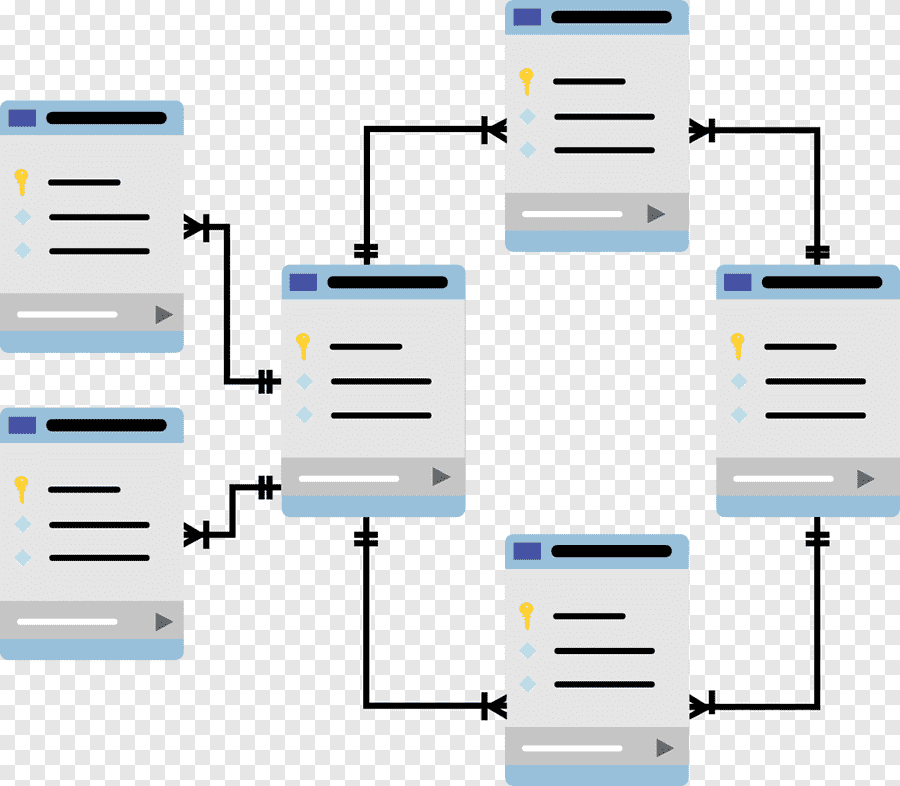
\includegraphics[width=14cm]{figures/rdb}
	\caption[1. melléklet]{Adatbázis ábra}
	\label{fig-melleklet1}
\end{figure}

\clearpage % Kényszerített oldalváltás a két melléklet között

% --- MÁSODIK MELLÉKLET (Elforgatott dokumentum) ---
\begin{figure}[p] % [p] = külön oldalra kerül
	\centering
	\begin{turn}{90}
		
\includegraphics[width=23cm]{figures/melleklet}
	\end{turn}
	\caption[2. melléklet]{Szkennelt dokumentum}
	\label{fig-melleklet2}
\end{figure}

\clearpage

\begin{thebibliography}{11}
\addcontentsline{toc}{chapter}{\bibname}

\bibitem{palermo2008} 
\textsc{Jeffrey Palermo}: \emph{The Onion Architecture: part 1}, 2008. \url{https://jeffreypalermo.com/2008/07/the-onion-architecture-part-1/}

\bibitem{gossman2005} 
\textsc{John Gossman}: \emph{Introduction to Model/View/ViewModel pattern for building WPF apps}, 2005.

\bibitem{dotnet10} 
\textsc{Microsoft}: \emph{.NET 10 and ASP.NET Core Documentation}, 2025. \url{https://learn.microsoft.com/en-us/dotnet/}

\bibitem{efcore} 
\textsc{Microsoft}: \emph{Entity Framework Core Documentation}, 2025. \url{https://learn.microsoft.com/en-us/ef/core/}

\bibitem{nextjs} 
\textsc{Vercel}: \emph{Next.js Documentation}, 2025. \url{https://nextjs.org/docs}

\bibitem{reactnative} 
\textsc{Meta}: \emph{React Native · A framework for building native apps using React}, 2025. \url{https://reactnative.dev/docs/getting-started}

\bibitem{postgresql} 
\textsc{PostgreSQL Global Development Group}: \emph{PostgreSQL 16 Documentation}, 2023. \url{https://www.postgresql.org/docs/16/index.html}

\bibitem{redis} 
\textsc{Redis}: \emph{Redis Documentation}, 2025. \url{https://redis.io/docs/}

\bibitem{minio} 
\textsc{MinIO}: \emph{MinIO High Performance Object Storage}, 2025. \url{https://min.io/docs}

\bibitem{tailwindcss} 
\textsc{Tailwind Labs}: \emph{Tailwind CSS Documentation}, 2025. \url{https://tailwindcss.com/docs}

\end{thebibliography}


\end{document}
